\documentclass[12pt, letterpaper]{article}
\usepackage[utf8]{inputenc}
\usepackage{graphicx}

\title{Rapport de projet : Compression d'image par la méthode Run-Length-Encoding}
\author{Chaolei Cai
\\
  \multicolumn{1}{
      p{.7\textwidth}}{\centering\emph{Université Paris Vincennes St-Denis\\
  UFR mathématiques, informatique, technologies sciences de l'information\\}
  L3 Informatique}
}
\date{\today}
\begin{document}


\begin{titlepage}
    \maketitle
\end{titlepage}

\tableofcontents

\section{Présentation du projet}
Ce document est mon rapport pour le projet 11 du cours d'algorithmique avancé enseigné par M.Bourdin.\\
Le sujet de mon projet est de mettre en place l'algorithme de Run-Length-Encoding(RLE)\\

%\begin{figure}
%    
\includegraphics[width=\linewidth]{img/L1.png}
%    \caption{Welcome page}
%    \label{fig:L1}
%\end{figure}


\subsection{Profile}
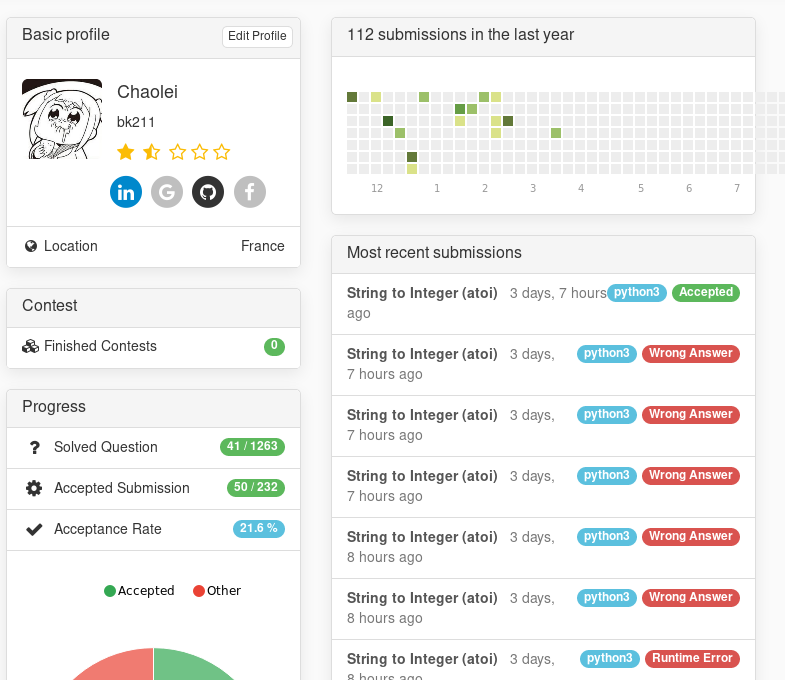
\includegraphics[width=\linewidth]{img/L6.png}


\end{document}
